\documentclass[lineno]{cls/jfm}

\usepackage{graphicx}
%\usepackage{epstopdf,epsfig}
%\usepackage{subfigure}%add
\usepackage{newtxtext}
\usepackage{newtxmath}
\usepackage{natbib}
\usepackage{hyperref}
\hypersetup{
    colorlinks = true,
    urlcolor   = blue,
    citecolor  = black,
}
\newtheorem{lemma}{Lemma}
\newtheorem{corollary}{Corollary}
\newcommand{\RomanNumeralCaps}[1]
\linenumbers


% {\MakeUppercase{\romannumeral #1}}

\title{Influence of Electric Potential Decay to the Impact Regimes of Droplets on a Hydrophobic Electrode}

\author{Ziqiang Ma\aff{1},
 \and Xinping Zhou\aff{1,2}
 \corresp{\email{JFMEditorial@cambridge.org}}}

\affiliation{\aff{1}School of Mechanical Science and Engineering, Huazhong University of Science and Technology, Wuhan 430074, PR China
\aff{2}State Key Laboratory of Intelligent Manufacturing Equipment and Technology, Huazhong University of Science and Technology, Wuhan 430074, China}

\begin{document}
\maketitle

\begin{abstract}
 Direct numerical simulations of \cite{popinet_gerris_2003}
\end{abstract}

\begin{keywords}
Authors should not enter keywords on the manuscript, as these must be chosen by the author during the online submission process and will then be added during the typesetting process (see \href{https://www.cambridge.org/core/journals/journal-of-fluid-mechanics/information/list-of-keywords}{Keyword PDF} for the full list).  Other classifications will be added at the same time.
\end{keywords}
%capillary flows, drops, contact lines

\section{Introduction}
\label{sec:headings}

The dynamics of droplet impact on solid surfaces is a classical problem in fluid mechanics, with various engineering applications, including inkjet printing, spray cooling, and microfluidic actuation. The interaction between inertia, surface tension, viscosity, and wettability gives rise to complex behaviors, such as spreading, retraction, rebound, or splashing. In recent years, the ability to actively modulate wettability through external stimuli has attracted significant interest, particularly via electrowetting-on-dielectric (EWOD). In EWOD systems, the apparent contact angle of a droplet can be dynamically controlled by applying an electric potential across a dielectric-coated electrode, enabling real-time tuning of droplet behavior. 

Previous studies have extensively investigated the role of electrowetting in modifying contact angle hysteresis, controlling spreading dynamics, and suppressing rebound. Most of these works, however, assume that the applied electric field is spatially uniform. In practical implementations--especially when thin electrodes with finite conductivity or localized voltage sources are employed--the electric potential may decay laterally along the substrate. This non-uniformity can lead to spatial gradients in wettability and contact angle, potentially altering the droplet impact regimes. Despite its physical relevance, the influence of electric potential decay on droplet dynamics has received little attention and remains poorly understood.

In this work, we study the impact of a millimetric water droplet on a hydrophobic substrate subject to a laterally decaying electric potential of the form $\phi(r) = \phi_0 e^{-\alpha r}$, where $\alpha$ is the electric potential decay constant. Using a dimensionless formulation, we investigate how this spatial variation in potential affects the contact angle distribution, impact-induced deformation, and rebound behavior. Furthermore, we extend our analysis to include time-harmonic potentials to examine the frequency-dependent response of the droplet under alternating fields. A combination of numerical simulation and phase-space classification is employed to delineate different behavioral regimes.

The paper is organized as follows. Section~\ref{sec:Problem and method} introduces the problem formulation and numerical methods. Section~\ref{sec:Results} presents a phase diagram and classification of electrowetting-induced wettability. The influence of electric potential decay on droplet dynamics is then examined, followed by an analysis of the frequency-dependent response of droplet behavior under time-varying electric potentials. Conclusions are drawn in Section~\ref{sec:Conclusion}.

\section{Problem and method}\label{sec:Problem and method}

\subsection{Governing equations and numerics models}

 \begin{figure}
  \centerline{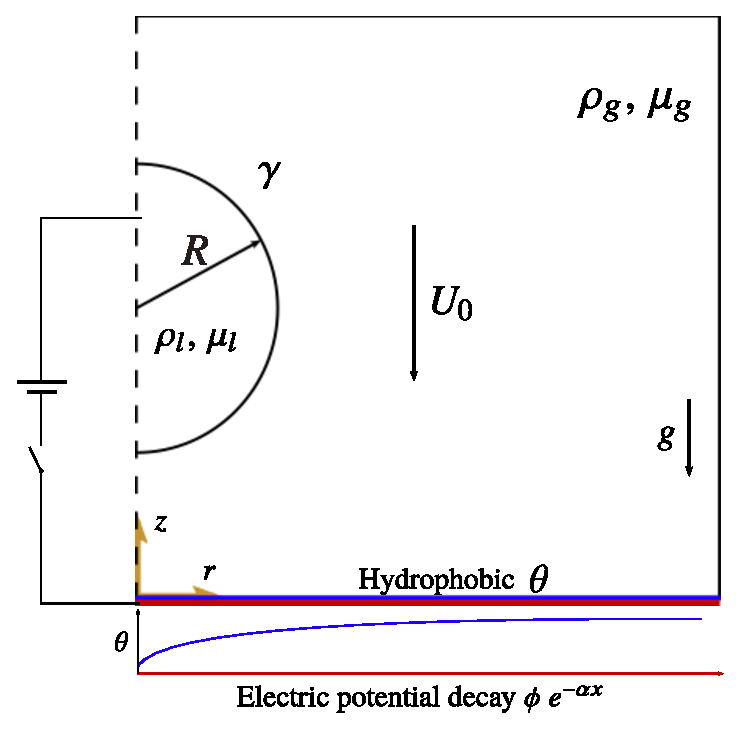
\includegraphics[width=0.5\textwidth]{fig/model.eps}}
  \caption{model}
 \label{fig:domain}
 \end{figure}

Consider a water droplet of diameter $D$ placed upon the substrate exhibiting electric potential decay $\phi e^{-\alpha r}$, where $\alpha$ is the electric potential decay constant. The droplet impacts the electrowetting surface with the velocity $U_0$. The density and viscosity are denoted by $\rho$ and $\mu$, with subscripts $l$ and $g$ indicating the liquid and the surrounding gas. In the electrowetting on dielectric (EWOD) phenomena under consideration, the wettability of substrate is varied by applied electric current. The variation of contact angle which is inducted by electrowetting can be described by the Young-Lippmann equation

\begin{equation}
	\cos(\theta_{\mathrm{ew}}) = \cos\theta_{\mathrm{s}} + \frac{\epsilon_0 \epsilon_r}{2 \gamma d} \phi^2 .
  \label{Young-Lippmann equation}
\end{equation}

\noindent $\theta_{\mathrm{s}}$ is the static contact angle, $\theta_{\mathrm{ew}}$ is the electrowetting induced contact angle, and $\gamma$ is the surface tension. $\epsilon_0$ is the vacuum's permittivity, $\epsilon_r$ and $d$ is the dielectric constant and dielectric thickness. Due to the electric potential decay, the contact angle at the wall exhibits a trend of being lower at the center and higher at the periphery. Figure \ref{fig:domain} shows the configuration of the water droplet in the domain for computations. 

The water droplet and surrounding fluid are controlled by the continuity and momentum equations for the incompressible fluids

\begin{equation}
  \nabla \cdot \mathbf{u} = 0,
  \label{continuity equation}
\end{equation}

\begin{equation}
  \rho(\partial_t \mathbf{u} + \mathbf{u} \nabla \cdot \mathbf{u})=-\nabla p + \nabla \cdot \mu (\nabla\mathbf{u}+\nabla^T\mathbf{u}) + \gamma \kappa \delta_s \mathbf{n} + \rho \mathbf{g} ,
  \label{momentum equation}
\end{equation}

\noindent where $p$ is the pressure, $\mathbf{g}$ is the gravity acceleration. A volume fraction function, denoted by $c$, is introduced to distinguish between the two immiscible fluid phases in the computational domain. Specifically, $c = 1$ corresponds to the liquid phase (water), and $c = 0$ corresponds to the gas phase (air). This function is constructed based on the known location of the interface. Since the density $\rho$ and viscosity $\mu$ are constant within each phase, their spatial distributions across the domain can be conveniently expressed in terms of $c$ as follows:

\begin{equation}
  \begin{aligned}
  \rho &= \rho_{g} + (\rho_{l} - \rho_{g})c, \\
  \mu  &= \mu_{g} + (\mu_{l} - \mu_{g})c,
  \end{aligned}
  \label{volume fraction function}
\end{equation}

\noindent where subscripts $l$ and $g$ denote the liquid and gas phases, respectively. The function $c$ thus implicitly tracks the interface and evolves in time according to the following advection equation:

\begin{equation}
  \partial_t c + \nabla \cdot (c \boldsymbol{u}) = 0,
  \label{advection equation}
\end{equation}

\noindent We nondimensionalize all variables using the diameter of the drop $D$. Therefore, the timescale is $\tau=\sqrt{\rho_l D^3 / \gamma}$, the velocity scale is $\sqrt{\gamma/\rho_l D}$, and the length scale is $D$. The three nondimensional parameters, the Ohnesorge number, the Weber number, the Bond number:

\begin{equation}
  Oh = \frac{\mu}{\sqrt{\rho \gamma D}}, We = \frac{\rho D U_0}{\gamma}, Bo = \frac{\rho g D^2}{\gamma} .
  \label{advection equation}
\end{equation}


\noindent We consider the effect of gravity by setting $Bo$ as a constant in all cases. And all the material properties the density ratio $\rho_g/\rho_l$, the viscosity ratio $\mu_g/\mu_l$ are typically defined as constants $1 \times 10^{-3}$ and $1.79 \times 10^{-2}$. Here, a Volume-of-Fluid (VOF) method of combining an adaptive quad spatial discretisation \citep{popinet_gerris_2003, popinet_accurate_2009,afkhami_mesh-dependent_2009,afkhami_transition_2018} is chosen to implement the electrowetting technique with dynamic contact angle model. 


When a sessile droplet equilibrium on the substreate, the static contact angle $\theta_s$ is the angle between the interface of droplet and the substrate surface. The dynamic contact angle $\theta_{\mathrm{D}}$ is implemented using the molecular kinetic theory (MKT) \citep{duvivier_toward_2013,cheng_numerical_2018,kumar_droplet_2024}. Using the theory, the dynamic contact angle $\theta_D$ and contact line velocity $v_{\mathrm{cl}}$ have the following relationship:

\begin{equation}
  v_{\mathrm{cl}} = 2 k_s^0 l \left (  \frac{h}{\mu V_m} \right ) \sinh{\left[ \frac{\gamma}{2 n k_B T} (\cos{\theta_{\mathrm{s}}} - \cos{\theta_D}) \right]}.
  \label{contact line velocity equation}
\end{equation}

\begin{table}
  \begin{center}
\def~{\hphantom{0}}
  \begin{tabular}{clr}
    Parameter          & Description                 & Value \\[3pt]
    $\epsilon_0$       & Vacuum permittivity         & $8.85 \times 10^{-12}~\mathrm{m}$ \\
    $\epsilon_r$       & Dielectric constant         & $2.6$ \\
    $k_s^0$       & Dielectric constant         & $4.5627 \times 10^{10}~\mathrm{s^{-1}}$ \\
    $l$           & Molecular displacement      & $5 \times 10^{-10}~\mathrm{m}$ \\
    $h$           & Planck constant       & $6.63 \times 10^{-34}~\mathrm{Js}$ \\
    $V_m$         & Molecular volume      & $3 \times 10^{29}~\mathrm{m^{3}}$ \\
    $k_B$         & Boltzmann constant    & $1.38 \times 10^{-23}~\mathrm{m^{3}}$ \\
    $T$           & Temperature           & $298.15~\mathrm{K}$ \\
    $d$           & Dielectric thickness  & $1 \times 10^{-5}~\mathrm{m}$ \\
  \end{tabular}
  \caption{Summary of operating parameters used for MKT model in the simulations.}
  \label{tab:parameters}
  \end{center}
\end{table}


\noindent The values of all reference parameters employed in the present study are summarized in Table~\ref{tab:parameters}. The contact line velocity is limited by the maximum for the dynamic contact angle of $180^\circ$ and the minimum for the dynamic contact angle of $0^\circ$:

\begin{equation}
  v_{\mathrm{cl} 180^\circ} = 2 k_s^0 l \left (  \frac{h}{\mu V_m} \right ) \sinh{\left[ \frac{\gamma}{2 n k_B T} (\cos{\theta_{\mathrm{s}}} + 1) \right]},
  \label{contact line velocity upper}
\end{equation}

\begin{equation}
  - v_{\mathrm{cl} 0^\circ} = 2 k_s^0 l \left (  \frac{h}{\mu V_m} \right ) \sinh{\left[ \frac{\gamma}{2 n k_B T} ( 1 - \cos{\theta_{\mathrm{s}}} ) \right]}.
  \label{contact line velocity lower}
\end{equation}


\noindent Although the contact line velocity $v_{\mathrm{cl}}$, can theoretically exceed both upper and lower limit, the numerical simulations are constrained to operate within the limits specified by Eqs.~\ref{contact line velocity upper} and \ref{contact line velocity lower}. Under reference conditions, the dynamic contact angle (DCA) is inferred from the prescribed contact line velocity by inverting the corresponding relation. The expression used to compute the DCA is given by

\begin{equation}
  \theta_{\mathrm{D}} = \cos^{-1} \left[ \cos \theta_{\mathrm{s}} - \left( \frac{2n k_B T}{\gamma} \sinh^{-1} \left( \frac{v_{\mathrm{cl}} \mu V_m}{2k_s^0 l h} \right) \right) \right].
  \label{dynamic contact angle}
\end{equation}


Electrowetting technique enables dynamic control of surface wettability by applying an electric potential across a conductive droplet. When the electric potential is established between the droplet and an underlying electrode, charges accumulate at the three-phase contact line. This localized buildup of electric charge leads to a reduction in the interfacial energy between the droplet and the substrate. The extent of contact angle modulation depends on the properties of the liquid, the characteristics of the substrate, and the parameters of the applied electric field in Eqs.~\ref{Young-Lippmann equation}. Accordingly, the relationship between the dynamic contact angle induced by electrowetting and contact line velocity is described by:

\begin{equation}
  \theta_{\mathrm{ED}} = \cos^{-1} \left[ \cos\theta_{\mathrm{s}} + \frac{\epsilon_0 \epsilon_r}{2 \gamma d} \phi^2 - \left( \frac{2n k_B T}{\gamma} \sinh^{-1} \left( \frac{v_{\mathrm{cl}} \mu V_m}{2k_s^0 l h} \right) \right) \right].
  \label{dynamic contact angle induced by electrowetting}
\end{equation}




\subsection{Problem setup and numerics validation}

 As shown in figure~\ref{fig:domain}, a spherical water droplet of diameter $D$ is initially positioned in close proximity to the lower boundary, which consists of a solid substrate subject to an applied electric potential. The droplet impacts the surface with a prescribed velocity $U_0$, and the dynamics are governed by the electrowetting-on-dielectric (EWOD) mechanism. Initially, the contact angle is static, with $\theta_{\mathrm{s}} = 90^\circ$. Upon actuation, the contact angle varies dynamically in response to the applied voltage, which is both spatially and temporally dependent. The applied voltage is defined as

\begin{equation}
  \phi(r,t) = \phi_0 \cos(2\pi f t) \cdot \mathrm{e}^{- \alpha r},
  \label{dynamic electric potential}
\end{equation}

\noindent where $\phi_0$ is the peak amplitude of electric potential, $f$ is the oscillation frequency, and $\alpha$ characterizes the radial decay of the electric potential, accounting for the influence of a uniform resistance on the potential distribution along the dielectric layer. The computational domain is taken as $8R \times 8R$ to ensure sufficient space for droplet deformation and spreading during impact and subsequent evolution. The bottom of the computational domain ($z = 0$) is a no-slip boundary condition, and the left ($r = 0$) is an axisymmetric boundary condition. All remaining boundaries of the computational domain are open boundary conditions.

Building upon earlier incompressible flow theories \citep{smith_air_2003, korobkin_trapping_2008}, \citet{mandre_precursors_2009} derived a criterion to assess the relevance of gas compressibility during high-velocity droplet impacts. Specifically, they introduced a non-dimensional compressibility parameter defined as the ratio between the ambient atmospheric pressure and a characteristic lubrication pressure in the gas layer:

\begin{equation}
  \epsilon = \frac{P_{\mathrm{atm}}}{\left(0.5 * D U_0^7 \rho_l^4 / \mu_g \right)^{1/3}},
  \label{compressibility equation}
\end{equation}

\noindent where $P_{\mathrm{atm}}$ is the ambient atmospheric pressure, and $\mu_g$ the gas viscosity. According to their analysis, gas compressibility becomes significant when $\epsilon^{-1} \gtrsim 3$. In light of this criterion, and supported by the conclusions of \citet{li_time-resolved_2015} and \citet{mandre_precursors_2009}, we neglect gas compressibility effects in the present study. The estimated range of the inverse compressibility parameter in our simulations is $\epsilon^{-1} \approx 0.1 \text{--} 2.0$, which remains well below the threshold for compressibility to play an important role. These values differ slightly from those in earlier studies due to variations in Ohnesorge ($Oh$) and Weber ($We$) numbers, but they still justify the assumption of incompressibility for the gas phase under the current impact conditions.

 \begin{figure}
  \centerline{\includegraphics[width=0.5\textwidth]{fig/Verity.pdf}}
  \caption{Comparison of drop spreading radius during impact process obtained from experiment data reported by \cite{sikalo_analysis_2002}.}
 \label{fig:verity}
 \end{figure}


To ensure the accuracy and reliability of the numerical model, simulation results are validated against experimental data reported by \citet{sikalo_analysis_2002}. Figure~\ref{fig:verity} presents the time evolution of the spreading radius of the droplet, normalized by its initial radius, as a function of the non-dimensional time. All physical parameters used in the simulation are consistent with those in the referenced experiment. In particular, the Weber number is $We = 44$, and the static contact angle is set to $100^\circ$, matching the experimental configuration. The simulation results exhibit excellent agreement with the experimental data, thereby demonstrating the validity of the computational model in capturing the essential physics of droplet impact and spreading dynamics.

 \begin{figure}
  \centerline{\includegraphics[width=0.5\textwidth]{fig/mesh.pdf}}
  \caption{Comparison of drop spreading radius during impact process obtained from simulations at $We=20$.}
 \label{fig:mesh}
 \end{figure}

For grid independence, we compare the spreading radius with time obtained from simulations, using different grid resolutions to assess the effect of varying grid sizes on the simulation accuracy. Figure \ref{fig:mesh} shows the finest grid sizes from low to high are $\Delta/D = 4.8 \times 10^{-3}$, $\Delta/D = 2.4 \times 10^{-3}$, and $\Delta/D = 1.2 \times 10^{-3}$ for the given computational domain. The orange dash line is the finest grid level $12$, the red line is the finest grid level $13$ and the blue dash line is the finest grid $14$. Despite these minor differences in the three levels, we notice that the middle grid size level reach the results are not significantly influenced by the grid resolution, while also accounting for the prohibitive computational costs involved. Thus, we choose the middle grid size level for all of our simulations.

\section{Results}\label{sec:Results}

In order to compare the dynamics of droplet motion, we first deployed droplets to impact on substrates with the same initial static contact angle, $\theta_{\mathrm{s}} = 90^\circ$. The droplets go through three distinct stages: spreading, retracting, and rebounding, before eventually detaching from the substrate. To actively control the contact angle during these dynamics, a voltage is applied between the conducting droplet and an underlying insulated electrode. This configuration, typical of the electrowetting-on-dielectric (EWOD) setup, consists of a hydrophobic dielectric layer that electrically isolates the droplet from the conductive substrate. When the electric field is activated, charges accumulate on the droplet side of the dielectric layer, forming a capacitor-like structure. This localized charge distribution results in a reduction of the interfacial energy near the contact line, thereby decreasing the apparent contact angle $\theta_{\mathrm{ED}}$ of the droplet. The variation of the contact angle $\theta_{\mathrm{ED}}$ with applied voltage is governed by the Young-Lippmann equation. To investigate the role of electric potential decay in electrowetting-induced wettability changes, we conduct droplet impact experiments at fixed dimensionless parameters, $Oh = 2.621 \times 10^{-3}$ and $Bo = 0.536$.

\subsection{Phase Diagram and Classification of Electrowetting-Induced Wettability}

When droplet impact the substrate with different electrowetting-induced wettability, it exhibits distinct dynamic reaction owing to voltage-induced variations in the equilibrium contact angle. Since the contact angle governs the balance of interfacial forces, the difference in wettability significantly influences the spreading, retraction, and rebound behaviour of the droplet. On a substrate with an equilibrium contact angle of $90^\circ$, the droplet follows the classical sequence of spreading, receding, and rebounding. At low impact velocities (i.e., low Weber numbers), the droplet may remain entirely separated from the substrate by a thin air layer, resulting in non-contact bouncing. At sufficiently high Weber numbers, the droplet undergoes splashing, with the emission of secondary droplets. To systematically characterise the influence of electrowetting, we construct a phase diagram in the applied voltage-Weber number plane that delineates the regimes of droplet impact behaviour under varying wettability conditions. 

 \begin{figure}
  \centerline{\includegraphics[width=0.8\textwidth]{fig/phase.pdf}}
  \caption{Phase diagrams of the motion state of a droplet impacting with the applied voltage varies obtained from simulations.}
 \label{fig:mesh}
 \end{figure}
 
 When a droplet impacts a solid wall at relatively high velocity, it typically exhibits splashing. For low-viscosity droplets, however, splashing behaviour is typically suppressed \citep{jian_two_2018}. Upon contacting the substrate, the droplet's kinetic energy undergoes rapid conversion into surface energy. This process drives spreading to a maximum radius. Subsequently, under the influence of significant surface energy potential, the droplet undergoes accelerated retraction. Capillary waves converging radially inwards from the spreading periphery focusing at the axisymmetric centre, thereby initiating vertical columnar jet formation. 

 The state of Complete rebound is noticed to exist widely in the range of $We$ number less than $5$. The bouncing mechanism is predicated on the persistence of an air film sustained at low impact velocities. This sub-micrometre air cushion dissipates kinetic energy and reverses the momentum of droplets. The droplets 




 \begin{figure}
  \centerline{\includegraphics[width=1.0\textwidth]{fig/dropA.pdf}}
  \caption{Phase diagrams of the motion state of a droplet impacting with the applied voltage varies obtained from simulations.}
 \label{fig:mesh}
 \end{figure}

\subsection{Influence of Electric Potential Decay on Droplet Behavior}

\subsection{Frequency-Dependent Response of Electrowetting-Induced Motion}


\section{Conclusion}\label{sec:Conclusion}



%\backsection[Supplementary data]{\label{SupMat}Supplementary material and movies are available at \\https://doi.org/10.1017/jfm.2019...}

%\backsection[Acknowledgements]{Acknowledgements may be included at the end of the paper, before the References section or any appendices. Several anonymous individuals are thanked for contributions to these instructions.}

\backsection[Funding]{This research was supported in part by the National Natural Science Foundation of China (No. 11972170). }

\backsection[Declaration of interests]{The authors report no conflict of interest.}

%\backsection[Data availability statement]{The data that support the findings of this study are openly available in [repository name] at http://doi.org/[doi], reference number [reference number]. See JFM's \href{https://www.cambridge.org/core/journals/journal-of-fluid-mechanics/information/journal-policies/research-transparency}{research transparency policy} for more information}

\backsection[Author ORCIDs]{Authors may include the ORCID identifers as follows.  Ziqiang Ma, https://orcid.org/0000-0003-3608-0199; Xinping Zhou, https://orcid.org/0000-0001-6340-5273}

%\backsection[Author contributions]{Authors may include details of the contributions made by each author to the manuscript'}

%\appendix

%\section{}\label{appA}
 

\bibliographystyle{bib/jfm}
\bibliography{bib/jfm}
%Use of the above commands will create a bibliography using the .bib file. Shown below is a bibliography built from individual items.

%\bibliographystyle{jfm2esam}
%\bibliography{jfm2esam}



%% End of file `jfm2esam.bib'.


\end{document}
